\chapter{言語的特徴量}

\section{a}

% 前後が役に立つことは分かっている。南条
% 金沢の人文献
% 周囲の言語を含めた特徴量を含めた

% TODO: 参考文献 音響学会15 金寺
NTCIR11 SpokenQuery\&Doc Formal-run の SQSCR SGS retrieval条件では,検索対象の文書に対し,周囲の文書を利用すると検索精度が向上する事が報告されている.金寺ら[]は音声内容検索において,検索対象文書の周囲に存在する文書に対し,シーンべクトルの線形補間を用いて音
声情報検索を行った結果,
検索性能が高いことが報告されている. \\
そこで本研究では,クエリ尤度を用いた検索モデルに対し,検索対象の周囲の単語を考慮することで,検索精度を改善する事を考案する.

\subsection{クエリ尤度の拡張}

% クエリ尤度と拡張
% 参考: http://www.fit.vutbr.cz/~imikolov/rnnlm/is2011_emp.pdf
クエリ尤度モデルにおいて,零確率問題を回避するために,式(\ref{eq_dirichlet})を用いて,ディリクレスムージングを行う.この式(\ref{eq_dirichlet})の文書コレクションから推定されたモデル $\theta_C$ に、周囲の文書の特徴量を付与することで、検索対象文書に適切な文書コレクションでスムージングを行い,検索性能を高める. \\
% TODO: コーパスに文書コレクションと同様にプラスαする事を説明する
本研究では,$\theta_C$ を推定するための文書モデルとして,キャッシュモデル,N-gramモデル,リカレントニューラルネットワーク言語モデルを検討する.Mikolovらは,キャッシュモデル,N-gramモデル(Kneser-Ney スムージング),リカレントニューラルネットワークモデルを用い,言語モデルを構築する事で言語モデルの評価基準であるパープレキシティを減少させることに成功している.そのため,本研究でも,言語的特徴量として有効であると推察できるキャッシュモデル,N-gramモデル,リカレントニューラルネットワーク言語モデルの3つモデルを用いる事で,検索精度がどのように変化するかを分析する.

% 参考: http://www.ar.media.kyoto-u.ac.jp/lab/bib/report/NEM-sdp07.pdf
\subsection{キャッシュモデルに基づく言語モデルの適応}
キャッシュモデルでは,単語 $w_n$ の直前の単語履歴をキャッシュ $H = \{ w_{n-|H|}, ..., w_{n-1}\} $ として記憶し,これに含まれる単語が再び使用される確率が高いと予測する.このキャッシュに基づく単語 $w_n$ の出現確率 $P_c(w_n|H)$ は式(\ref{cache})によって与えられる. ただし,$|H|$ は単語履歴 $H$ の長さ, $\delta$ はクロネッカーのデルタである.

\begin{equation}
		P_c(w_n|H) = \frac{1}{|H|} \sum_{w_h \in H} \delta (w_n, w_h)
    \label{cache}
\end{equation}

% 参考: http://www.cl.cs.titech.ac.jp/~fujii/paper/asj2002akiba.pdf
\subsection{N-gramとスムージング}

N-gram言語モデルでは、学習データに現れない単語列を扱うため、種々の平滑化(スムージング)手法が適用される。スムージングの一つとして,バックオフ・スムージングでは、高次のN-gramが存在しない場合、低次のN-gramで代用する。

\subsection{単語連接を重視したバックオフ平滑化手法}
バックオフ・スムージングの一般式は次のように表される。

\begin{equation}
		P(w_i|w_{i-n+1}^{i-1}) = 
    \begin{cases} 
        d_{w_{i-n+1}^i} P_{ML}(w_i|w_{i-n+1}^{i-1}) & C(w_{i-n+1}^{i-1}) > 0\\ 
        \alpha(w_{i-n+1}^{i-1})P(w_i|w_{i-n+2}^{i-1}) & C(w_{i-n+1}^{i-1}) = 0
    \end{cases} 
    \label{ngram_smoosing1}
\end{equation}

ここで $d$, $P_{ML}$, $\alpha$は、それぞれ、ディスカウント係
数、最尤推定によるN-gram確率、確率の総和を1とするための正規化係数である。

\subsection{Kneser-Ney スムージング}
KneserとNey[3]は、絶対法[4]を拡張した平滑化手法を示している
純粋に平滑化手法として他の手法と比べた場合でも、英語に適用した例で優れた性能を示すことが報告されている[2]。Kneser-Neyスムージングでは、高次のN-gram確率が利用できない(信頼できない)場合に使用する低次の確率として、最尤推定による確率 $P_{ML} (w_i|w_{i-n+1}^{i-1})$ の代わりに次の値 $P_{KN} (w_i|w_{i-n+1}^{i-1})$ を用いる.

\begin{equation}
		P_{KN} (w_i|w_{i-n+1}) = \frac{|\{w_{i-n}|C(w_{i-n+1}^{i-1}) > 0\}|}{\sum_{w_i} |\{w_{i-n}|C(w_{i-n+1}^{i-1}) > 0\}|} 
    \label{ngram_smoosing2}
\end{equation}

Kneser-Neyスムージングでは、長さ $N$ のN-gramについて, $n  <  N$ である全ての $n$ に対し,$P_{KN} (w_i|w_{i-n+1}^{i-1})$ を用いる。

% 参考: 複数の文脈長を考慮したリカレントニューラルネットワークに基づく言語モデル
\subsection{リカレントニューラルネットワーク言語モデル}
リカレントニューラルネットワークに基づく言語モデル(RNNLM)は,入力層 $x$ ,潜在層 $s$ ,出力層 $y$ から構成されるニューラルネットワークに基づく言語モデルであり,潜在層 $s$ に文脈を考慮するためのフィードバック構造をもつ. 入力層 $x(t)$は,時刻 $t$ における単語の1-of-K表現 $w(t)$ と直前の時刻 $t−1$
の潜在層 $s(t−1)$ から成り,式1で表される.

\begin{equation}
		x(t) = [w(t)^T s(t-1)T]T
    \label{rnn1}
\end{equation}

入力 $x(t)$ は潜在層 $s(t)$ へ変換され,出力層 $y(t)$ で次の時刻 $t+1$ に現れる単語の生起確率が算出される.

\begin{equation}
		s_j(t) = f(\sum_i x_i(t) u_{ji})
    \label{rnn2}
\end{equation}

\begin{equation}
		y_k(t) = g(\sum_j s_i(t) v_{kj})
    \label{rnn3}
\end{equation}

ただし, $U=(uji)$, $V=(vkj)$はそれぞれ入力層 $x$ と潜在層 $s$との間の重みパラメータ,潜在層 $s$
と出力層 $y$ との間の重みパラメータで, $f(·)$ はシグモイド関数, $g(·)$ はソフトマックス関数である.
RNNLMは時刻tの次に予測すべき単語 $w(t+1)$を教師信号としバックプロパゲーションによる学習を行なう.特に,潜在層のフィードバック構造を時間方向に展開しバックプロパゲーションを行なうことで長期的な文脈情報を学習する(BPTT).モデルの訓練方法の詳細については,[1,3]を参照されたい.

% TODO: RNNの利用方法を講演単位で学習してる。

\section{評価実験}
\subsection{実験条件}

% 認識結果クエリkaldiの音声認識結果
% ngramは3にしてる
% RNNは講演全体kaldiのみ学習してる。
% キャッシュモデルの長さは100
% ディリクレスムージングのパラメーターはu=320 v=10


% NTCIR12の実験の詳細をどこかに掲載する
% Juliusの音声認識結果とkaldiの音声認識結果の精度
% の違いにおけるMAP値の変化を調べるために,実験を行う.実験でははまず,NTCIR12のformal-runクエリに対して,JuliusとKaldiでそれぞれ認識された検索対象文書とクエリを比較,コンテンツとしてマッチする文書をシステムが抽出する.また,書き起こしの検索文書よるMAP値も,比較のため提示する.
% クエリの音声認識結果はJuliusの認識結果を利用する.文書の特徴量としてはクエリ尤度モデルにディリクレスムージングを施したものを利用し,そのときのMAP値を両者で比較する.

\subsection{実験結果}

% 表1より,MAP値はJuliusの音声認識文書,Kaldiの音声認識文書,書き起こし文書の順でMAP値が上昇していることが分かり,Juliusより生成された文書を利用するよりも,Kaldiを用いた文書を利用したほうが,MAP値がよいことが確認できた.

% \begin{table}
%     \centering
%     \caption{書き起こし文書と認識文書を用いたときのMAP値}
%     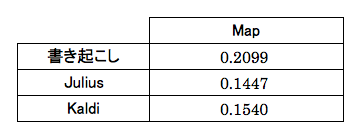
\includegraphics[width=7cm]{./image/write_julius_kaldi.png}
%     \label{query_set}
% \end{table}
